% !Mode:: "TeX::UTF-8"
\documentclass[myposter,portrait]{sciposter}

%% uzitocne package
\usepackage{multicol}
\usepackage{color}
\usepackage{graphicx}

%% znaky s diakritikou
\usepackage[utf8]{inputenc}
\usepackage[T1]{fontenc}
% \usepackage[slovak]{babel} % slovenske delenie slov

\usepackage{amsmath}
\usepackage{amsthm}
\usepackage{cite} %bibtex
\usepackage{colortbl} %for \rowcolor command
\usepackage{eucal} %for nice letters like \mathcal{A}
\usepackage{lmodern} %spolu s T1 smooth font!
\usepackage{lscape}
\usepackage{mathtools}
\usepackage{pdfpages}
\usepackage{pgfplots}
\usepackage{multirow}
\usepackage[rightcaption]{sidecap}
\usepackage{bm}

\usepackage{enumitem}
\usepackage{tikz}

\usetikzlibrary{decorations.pathreplacing}
\usetikzlibrary{shapes,fit,calc,shadows,plotmarks}

%---------------------------------------------------------------------
%   various settings
%---------------------------------------------------------------------

\definecolor{tablehead}{RGB}{238,233,233} %nice smooth grey
\definecolor{algcolor}{RGB}{0,0,0}
\definecolor{inalgcolor}{RGB}{0,0,0}
\definecolor{lstcolor}{RGB}{238,233,233}

\setlength{\parindent}{0pt} %we don't need no indentation

\graphicspath{{./pics/}} %picture dir

\setlist{nolistsep} %so that lists have normal spacing

\colorlet{city-clr}{green!70!black}
\colorlet{elcon-clr}{red}
\colorlet{event-clr}{blue}
\colorlet{waiting-clr}{olive}
\colorlet{cmt-clr}{gray}
\colorlet{oracle-clr}{orange!30}
\colorlet{algsec-clr}{black!50!red}

\renewcommand{\arraystretch}{1.1} %spacing of table rows


%% definicia farieb
\definecolor{mainCol}{rgb}{0.91,0.82,0.74} % farba pozadia posteru
\definecolor{sectionCol}{rgb}{0,0,0} % farba nadpisu
\definecolor{textCol}{rgb}{0.2,0,0} % farba hlavneho textu
\definecolor{BoxCol}{rgb}{1,1,0.8} % farba boxu okolo nadpisov

\def\mysection#1{
{\color{sectionCol}\section*{\sc\bfseries #1}}}

\interfootnotelinepenalty=10000

\newcommand{\inputTikZ}[1]{%
    \beginpgfgraphicnamed{#1-external}%
    \input{#1.tikz}%
    \endpgfgraphicnamed%
}	

\usepackage{eso-pic}
\newcommand\BackgroundPic{%
\put(-35, 35){%
\parbox[b][\paperheight]{\paperwidth}{%
\vfill
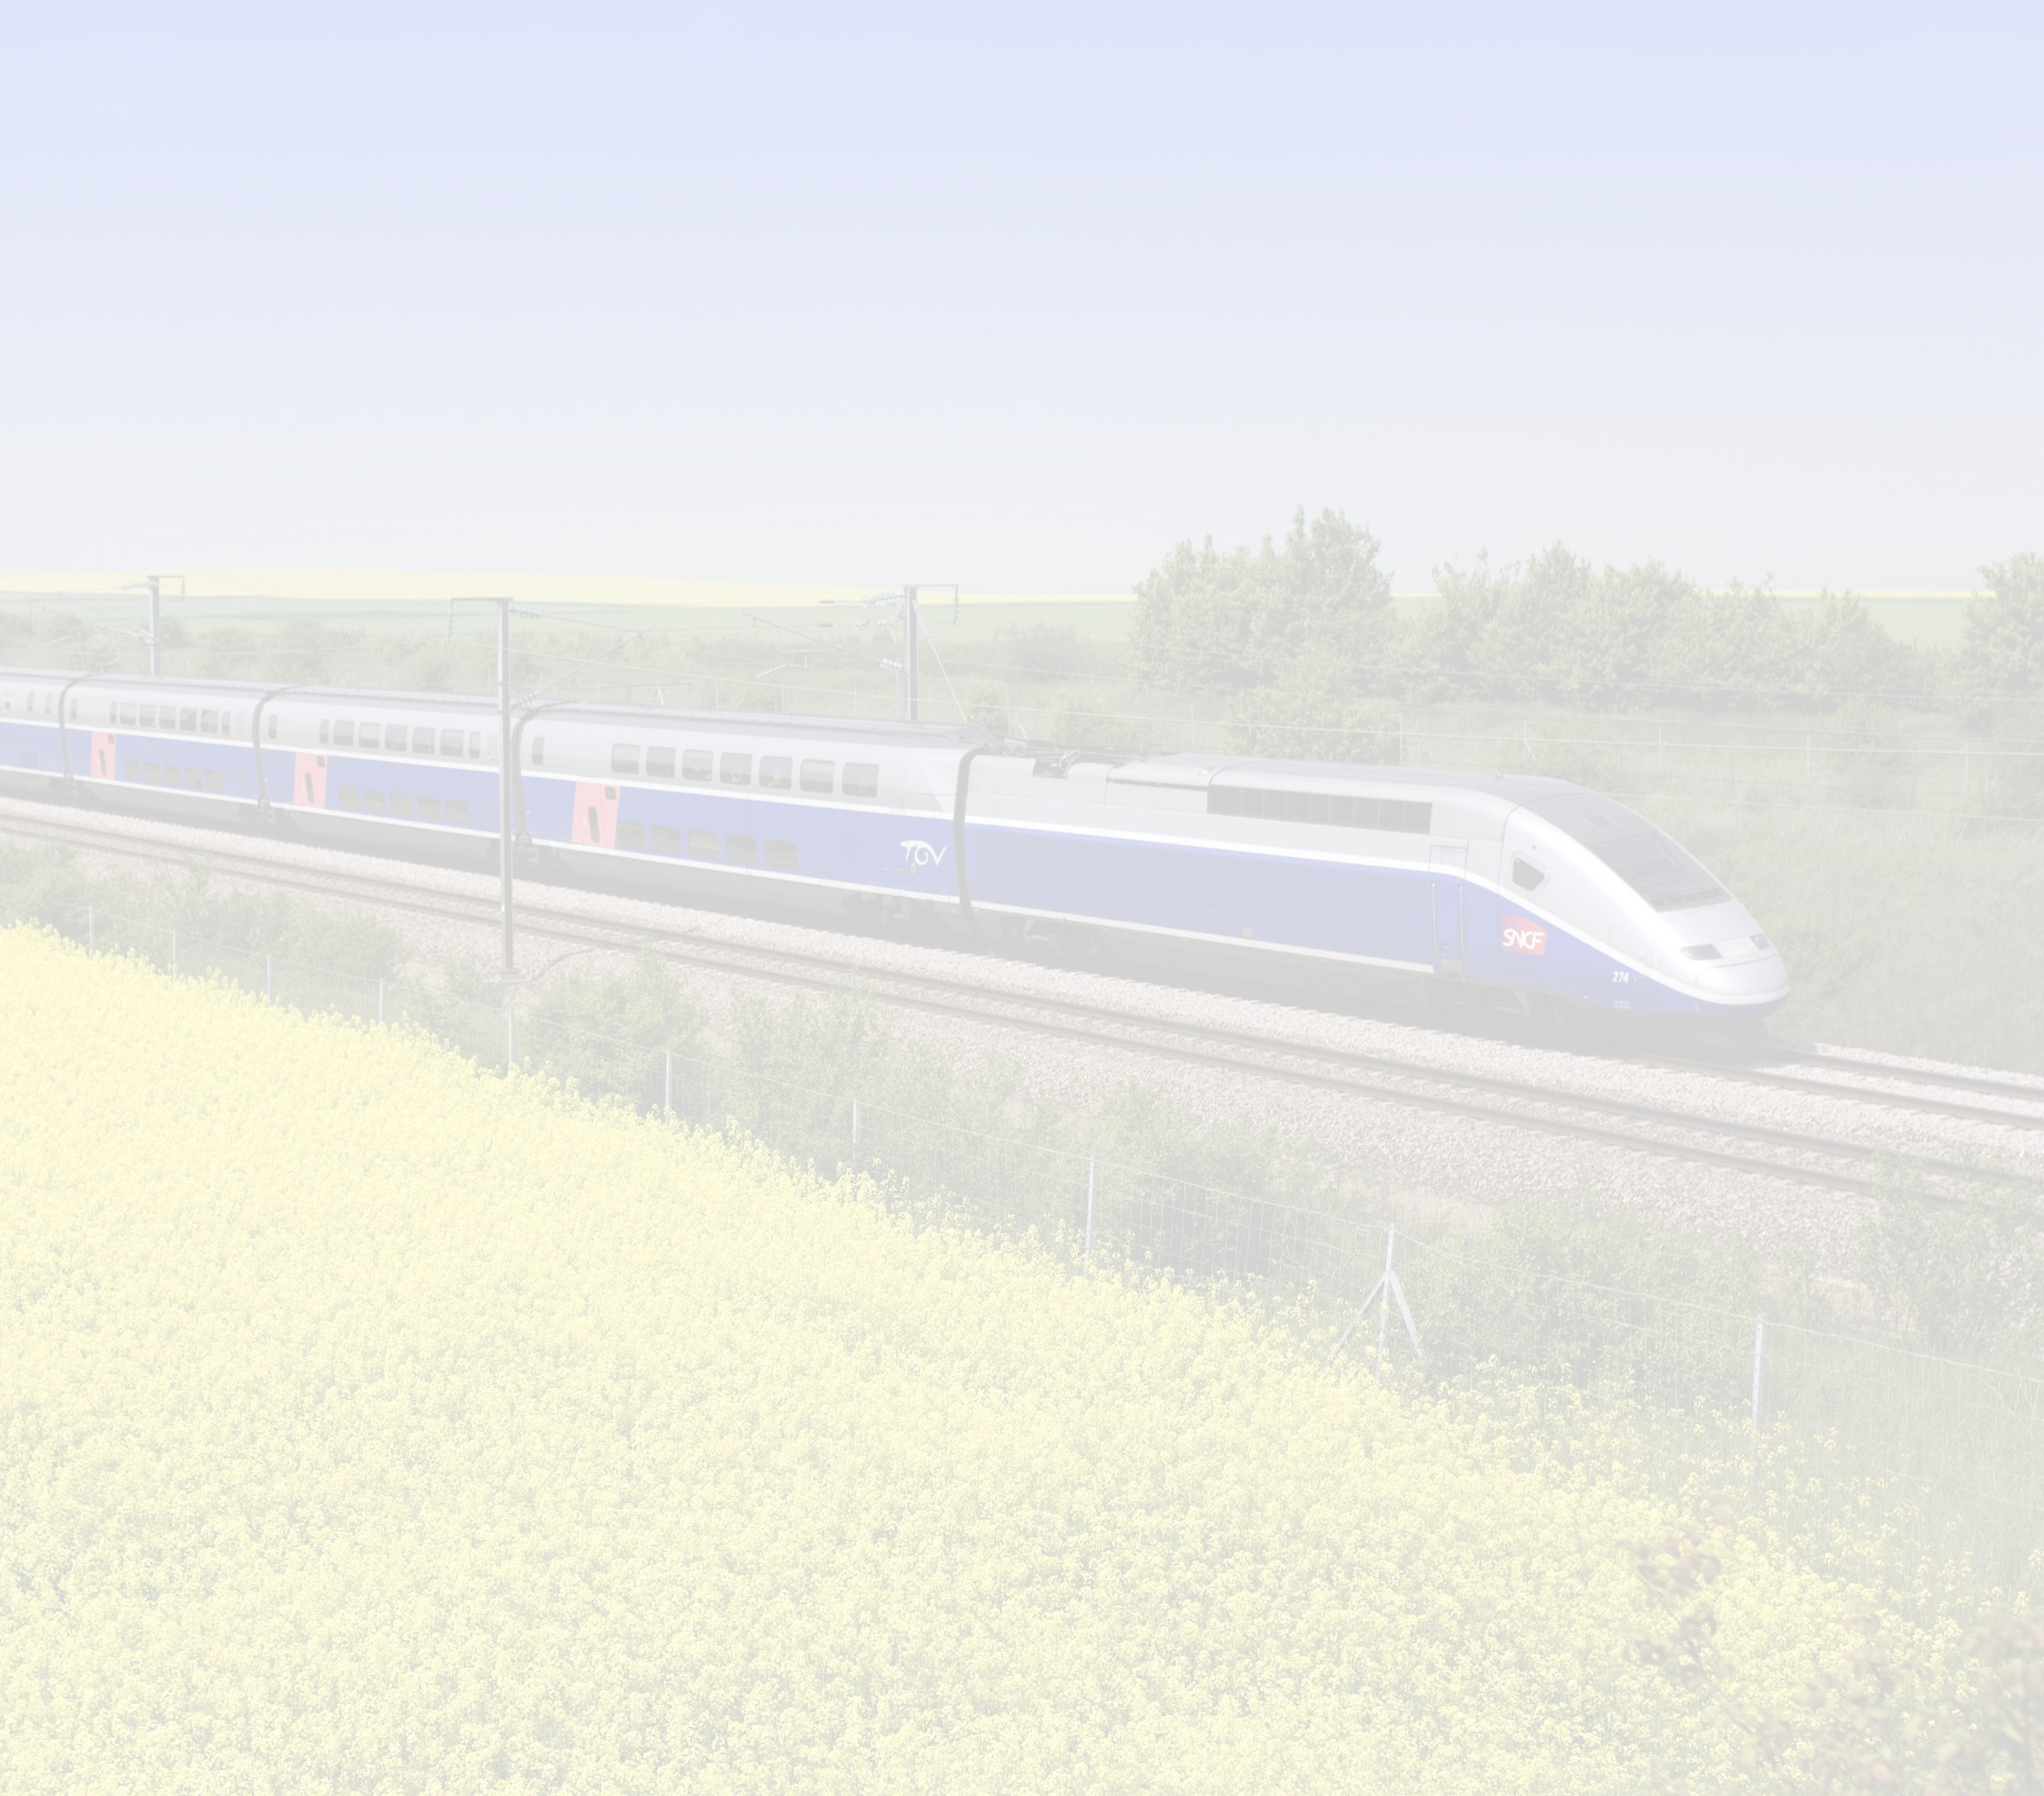
\includegraphics[width=\paperwidth,height=\paperheight]{tgv.jpg}%
\vfill
}}}

%---------------------------------------------------------------------
%   header
%---------------------------------------------------------------------

\begin{document}
\AddToShipoutPicture*{\BackgroundPic}
\setlength{\logowidth}{15cm}
\setlength{\titlewidth}{\textwidth}
\addtolength{\titlewidth}{-\logowidth}
\rightlogo[0.9]{fmfilogo-farebne}
\useleftlogofalse

\color{textCol}

\title{Underlying shortest paths in timetables}
\author{František Hajnovič$^1$\\
	Supervisor: Rastislav Královič$^1$}
\institute{
$^1$ Katedra informatiky, 
FMFI UK, Mlynská Dolina, 842~48~Bratislava}

\maketitle

%---------------------------------------------------------------------
%   poster
%---------------------------------------------------------------------

\begin{multicols*}{3}

\mysection{Introduction}

	We introduce methods to speed-up optimal connection queries in timetables based on pre-computing paths that are worth to follow. We present two methods:
	\begin{itemize}
		\item \textit{USP-OR} - very fast, but space consuming
		\item \textit{USP-OR-A} - fast, less space consuming
	\end{itemize}
	And we compare the methods to:
	\begin{itemize}
		\item \textit{Time-dependent Dijkstra}~\footnote{Implemented in $\mathcal{O}(m + n \log n)$ using Fibonacci heap priority queues~\cite{sommerthesis10}} - slowest, but least space consuming
	\end{itemize}
	\hspace{\fill}
	
	We define the most common terms:
	\begin{itemize}
		\item \textbf{Timetable} - a set of \textbf{elementary connections}~\cite{timetablemodelsalgs07} (see figure~\ref{fig:ttug} for an example)
		\item \textbf{Connection} - a valid sequence of elementary connections (may include also some waiting)
		\item \textbf{Underlying graph} of the timetable - nodes are the cities and there is an arc between two cities if some el. connection connects them.
	\end{itemize}

	\begin{figure}[htb]
	\centering
	\makebox[0pt][c]{
	\begin{minipage}{0.45\textwidth}
    	\centering
        \begin{tabular}{c|c|c|c}
        %legend
            \rowcolor{tablehead}
            \multicolumn{2}{>{\columncolor{tablehead}}c|}{\textbf{Place}} & \multicolumn{2}{>{\columncolor{tablehead}}c}{\textbf{Time}} \\
			\hline
           	\rowcolor{tablehead}
            \textbf{From} & \textbf{To} & \textbf{Departure} & \textbf{Arrival} \\
		%data
			\hline
            \textcolor{city-clr}{A} & \textcolor{city-clr}{B} & 10:00 & 10:45 \\
			\textcolor{city-clr}{B} & \textcolor{city-clr}{C} & 11:00 & 11:30 \\
			\textcolor{city-clr}{B} & \textcolor{city-clr}{C} & 11:30 & 12:10 \\
			\textcolor{city-clr}{B} & \textcolor{city-clr}{A} & 11:20 & 12:30 \\
			\textcolor{city-clr}{C} & \textcolor{city-clr}{A} & 11:45 & 12:15 \\
		\end{tabular}
	\end{minipage}
	\hspace{1cm}
	\begin{minipage}{0.45\textwidth}
        \centering
		\inputTikZ{./tikzpics/ug}
	\end{minipage}
	}
	\caption{\label{fig:ttug} A timetable and its underlying graph}
	\end{figure}
	
	\begin{itemize}
		\item \textbf{Underlying shortest path} (USP) - every path $p$ in the underlying graph, such that for some optimal connection $c^{*}$: $path(c^{*}) = p$ (function $path$ extracts the sequence of cities visited by the connection, see figure~\ref{fig:pathfunc}).
	\end{itemize}
	
	\begin{figure}[h!]
		\begin{center}
			\inputTikZ{./tikzpics/pathfunc}
		\end{center}
		\caption{\label{fig:pathfunc} The $path$ function gets the underlying path from a connection.}
	\end{figure}
	
	The timetables we used for testing are real datasets and they had the following properties:
	\begin{itemize}
		\item Their underlying graphs were sparse ($m \leq n \log n$, $n$ = number of cities)
		\item Average optimal connection was generally up to $\sqrt{n}$ 
		\item Average number of USPs between two cities was a small and constant (or slightly increasing with $n$)
	\end{itemize}
	\hspace{\fill}

\mysection{\textit{USP-OR}}

	Our first method, called \textit{USP-OR} (\textbf{USP} \textbf{or}acle), is based on pre-computing USPs between every pair of cities. Then, upon a query from $x$ to $y$ at time $t$ we consider one by one the computed USPs between $x$ and $y$ and perform a reverse operation to the $path$ function - $expand(p)$ where $p$ is an USP. The $expand$ function simply follows the sequence of cities in $p$ and from each of them it takes the first available el. connection to the next one, constructing one by one a connection from $x$ to $y$. 
	
	\begin{table}[h!]
		\centering
		\begin{tabular}{l|c|c|c|c}
		%legend
			\cellcolor{oracle-clr} \textit{\textbf{USP-OR}} & \cellcolor{oracle-clr} $\bm{prep}$ & \cellcolor{oracle-clr} $\bm{size}$ & \cellcolor{oracle-clr} $\bm{qtime}$ & \cellcolor{oracle-clr} $\bm{stretch}$ \\
		%data
			\hline
			\cellcolor{oracle-clr} \textbf{Our timetables} & $\mathcal{O}(hn^{2} \log n)$ & $\mathcal{O}(n^{2.5})$ & avg. $\mathcal{O}(\sqrt{n})$ & $1$ \\
		\end{tabular}
		\caption{\label{tab:uspor} Preprocessing time/size, query time and stretch (1 = exact answers) for \textit{USP-OR}}
	\end{table}	

\mysection{\textit{USP-OR-A}}

	To decrease the space complexity, in \textit{USP-OR-A} (\textbf{USP} \textbf{or}acle with \textbf{a}ccess nodes) we compute USPs only among cities from a smaller set - called \textbf{access node set} (AN set $\bm{\mathcal{A}}$). On a query from $x$ to $y$ at time $t$, we do:
	\begin{itemize}
		\item \textit{Local front search}: a local search in the neighbourhood of $x$ up to $x$'s local access nodes (LANs)
		\item \textit{Inter-AN search}: expand all USPs between $x$'s LANs and $y$'s back LANs
		\item \textit{Local back search}: a local search from $y$'s back LANs to $y$, restricted to $y$'s back neighbourhood
	\end{itemize}		

	\begin{figure}[h!]
		\begin{center}
			\inputTikZ{./tikzpics/uspora}
		\end{center}
	\end{figure}
	
	How to choose a good access node set?
	\begin{itemize}
		\item Solve optimally $\rightarrow$ NP-complete (reduction of minimal set cover)
		\item Heuristic approach $\rightarrow$ algorithm \textit{Locsep} (AN set made out of nodes that are good local separators)
	\end{itemize}
	
	\begin{figure}[htb]
	\centering
	\makebox[0pt][c]{
	\begin{minipage}{0.45\textwidth}
    	\centering
        \inputTikZ{./tikzpics/locsep}
	\end{minipage}
	\hspace{1cm}
	\begin{minipage}{0.45\textwidth}
        \caption{\label{fig:locsep} To evaluate the node's suitability to be an access node, we see what would happen to the reachability in its surroundings if we select it to the AN set.}
	\end{minipage}
	}
	\end{figure}	
	
	\begin{table}[h!]
		\centering
		\begin{tabular}{l|c|c|c|c}
		%legend
			\cellcolor{oracle-clr} \textit{\textbf{USP-OR-A + Locsep}} & \cellcolor{oracle-clr} $\bm{prep}$ & \cellcolor{oracle-clr} $\bm{size}$ & \cellcolor{oracle-clr} $\bm{qtime}$ & \cellcolor{oracle-clr} $\bm{stretch}$ \\
		%data
			\hline
			\cellcolor{oracle-clr} \textbf{Our timetables} & $\mathcal{O}(\delta n^{2.5})$ & $\mathcal{O}(n^{1.5})$ & avg. $\mathcal{O}(\sqrt{n} \log n)$ & $1$ \\
		\end{tabular}
	\end{table}

\mysection{Performance}

	We measured:
	\begin{itemize}
		\item \textbf{Speed-up} - how many times faster is the algorithm against the Time-dependent Dijkstra
		\item \textbf{Size-up} - how many times more memory is needed then to store the timetable itself
	\end{itemize}
	
	\begin{table}[h!]
        \centering
		\begin{tabular}{c|c|c|c|c|c}
		%legend
			\rowcolor{tablehead}
			 & \textbf{Dataset} & \textit{cpsk} & \textit{sncf} & \textit{gb-coach} & \textit{gb-tr} \\
			\rowcolor{tablehead}
			 & \textbf{Time range} & (1 day) & (1 day) & (1 week) & (1 week) \\			
		%data
			\hline
			\cellcolor{tablehead}  & \cellcolor{tablehead} $\bm{n}$ & 700 & 1000 & 1000 & 700 \\
			\cellcolor{tablehead} & \cellcolor{tablehead} \textbf{Speed-up} & 1 & 1 & 1 & 1 \\
			\multirow{-3}{*}{\textit{USP-OR}} \cellcolor{tablehead} & \cellcolor{tablehead} \textbf{Size-up} & 1 & 1 & 1 & 1 \\
			\hline
			\cellcolor{tablehead}  & \cellcolor{tablehead} $\bm{n}$ & 1905 & 2645 & 3915 & 2575 \\
			\cellcolor{tablehead} & \cellcolor{tablehead} \textbf{Speed-up} & 1 & 1 & 1 & 1 \\
			\multirow{-3}{*}{\textit{USP-OR-A}} \cellcolor{tablehead} & \cellcolor{tablehead} \textbf{Size-up} & 1 & 1 & 1 & 1 \\
		\end{tabular}
		\caption{\label{tab:speedup} Speed-ups and size-ups of \textit{USP-OR} and \textit{USP-OR-A} with \textit{Locsep}. Datasets from \textit{cp.sk}, SNCF (French railways) and Great Britain coaches and trains.}
	\end{table}
		
	\begin{figure}[H]
	    \centering
	    \inputTikZ{./tikzpics/plot_uspr_sncf_size}
	    \caption{\textbf{Query time} of \textit{USP-OR-A} with \textit{Locsep} compared to TD Dijkstra on the \textit{\textbf{sncf}} dataset. \textbf{Changing $\bm{n}$}.}
	    \label{plot:uspr-sncf-size}  
    \end{figure}
    
    \begin{figure}[H]
	    \centering
	    \inputTikZ{./tikzpics/plot_uspr_gbcoach_size}
	    \caption{\textbf{Query time} of \textit{USP-OR-A} with \textit{Locsep} compared to TD Dijkstra on the \textit{\textbf{gb-coach}} dataset. \textbf{Changing $\bm{n}$}.}
	    \label{plot:uspr-sncf-size}  
    \end{figure}	

\bigskip 
 

%% zoznam literatury
\bibliographystyle{apalike}
\bibliography{bibl}

\end{multicols*}
\end{document}

